\documentclass[oupdraft]{bio}
% \usepackage[colorlinks=true, urlcolor=citecolor, linkcolor=citecolor, citecolor=citecolor]{hyperref}
\usepackage{url}
\usepackage{longtable}
\usepackage{multirow}
\usepackage[T1]{fontenc}
\usepackage[utf8]{inputenc}
\usepackage[table]{xcolor}
\usepackage{caption}

\usepackage{tikz}
\usetikzlibrary{shapes}
\usepgflibrary{plotmarks}
\usetikzlibrary{plotmarks}


\newcommand{\mysquare}[1]{\tikz{\node[draw=#1,fill=#1,rectangle,minimum
width=0.18cm,minimum height=0.18cm,inner sep=0pt] at (0,0) {};}}

\newcommand{\mycircle}[1]{\tikz{\node[draw=#1,fill=#1,circle,minimum
width=0.2cm,minimum height=0.2cm,inner sep=0pt] at (0,0) {};}}

\newcommand{\mystar}[1]{\tikz{\node[draw=#1,fill=#1,star,minimum
width=0.2cm,minimum height=0.2cm,inner sep=0pt] at (0,0) {};}}

\newcommand{\mytriangle}[1]{\tikz{\node[draw=#1,fill=#1,isosceles
triangle,isosceles triangle stretches,shape border rotate=90,minimum
width=0.2cm,minimum height=0.2cm,inner sep=0pt] at (0,0) {};}}

% Add history information for the article if required
%\history{Received August 1, 2010; revised October 1, 2010; accepted for publication November 1, 2010}

\begin{document}

% Title of paper
\title{It's all About Balance: Propensity Score Matching in the Context of Complex Survey Data}

% List of authors, with corresponding author marked by asterisk
\author{DAVID LENIS$^\ast$\\
% Author addresses
\textit{Department of Biostatistics, Johns Hopkins Bloomberg School of Public Health, Baltimore, MD 21205, USA}\\
% E-mail address for correspondence
{dlenis@jhsph.edu}\\
TRANG QUYNH NGUYEN\\
\textit{Department of Mental Health, Johns Hopkins Bloomberg School of Public Health, Baltimore, MD 21205, USA}\\
NIANBO DONG\\
\textit{Department of Educational, School and Counseling Psychology, College of Education, University of Missouri, Columbia, MO 65211, USA}\\
ELIZABETH A. STUART\\
\textit{Departments of Mental Health, Biostatistics, and Health Policy and Management, Johns Hopkins Bloomberg School of Public Health, Baltimore, MD 21205, USA}}

% Running headers of paper:
\markboth%
% First field is the short list of authors
{D. Lenis and others}
% Second field is the short title of the paper
{Propensity Score Matching with Complex Survey Data}
\maketitle

% Add a footnote for the corresponding author if one has been
% identified in the author list
\footnotetext{To whom correspondence should be addressed.}

\begin{abstract}
{Many research studies aim to draw causal inferences using data from large, nationally representative survey samples, and many of these studies use propensity score matching to make those causal inferences as rigorous as possible given the non-experimental nature of the data. However, very few applied studies are careful about incorporating the survey design with the propensity score analysis, which may mean that the results do not  generate population inferences. This may be because few methodological studies examine how to best combine these methods. Furthermore, even fewer of them investigate different non-response mechanisms. This study examines methods for handling survey weights in propensity score matching analyses of survey data under different non-response mechanisms. Our main conclusions are: (1) whether the survey weights are incorporated in the estimation of the propensity score does not impact estimation of the population treatment effect, as long as good population treated-comparison balance is achieved on confounders, (2) survey weights must be used in the outcome analysis, and (3) the transferring of survey weights (i.e., assigning the weights of the treated units to the comparison units matched to them) can be beneficial under certain non-response mechanisms.}
{Propensity Score; Propensity Score Matching, PATT, SATT, PATE, SATE, Complex Survey Data, Survey Weights, Non-response.}
\end{abstract}


\section{Introduction}
\label{S1}
\subsection{Background}
\label{S1.1}
Non-experimental data are increasingly used to estimate the causal effects of an exposure or intervention (hereafter `treatment'), especially when a randomized trial is infeasible or unethical. More often than not, the interest is in causal effect estimates that apply to an entire target population, not just the data sample. These interests combined call using data that inform about the target population and statistical methods that ensure accurate inferences. Two tools for these purposes are large-scale nationally representative datasets and propensity score methods.

Large-scale complex surveys are widely used and usually have a well-defined target population. The sampling framework may be complicated, and the sampling probabilities vary depending on the sampling of sub-populations. When making inferences about the target population, survey weights and other survey design elements should be correctly used in data analysis; otherwise parameter estimates may not relate to the original target population of the survey
-- see \citet{hansen1983evaluation}, \citet{korn1995analysis}, \citet{korn1995examples} and \citet{little2003bayesian}.


The causal inference framework introduced by \citet{rubin1974estimating} extended the estimation of causal effects to non-experimental studies.  Since propensity scores (i.e.,  the probability of receiving treatment given a set of observed covariates) were introduced by \citet{rosenbaum1983central}, a wide range of methods have been developed to estimate treatment effects in non-experimental studies (e.g., propensity score based matching, weighting, and subclassification).

In particular, propensity score matching estimators have been widely used in the context of non-experimental studies. Matching methods help reduce bias in the estimation of causal effects \citep{rubin1973matching}, and are intuitive and relatively easy to implement. Standard propensity score matching methods, however, do not give guidance on how to incorporate survey weights, and conceptually it is somewhat unclear how to do so. As a consequence, researchers using propensity score matching often do not incorporate the complex survey design \citep[e.g.,][]{morgan2008propensity}. This paper aims to provide guidance on propensity score matching using complex survey data to ensure that the estimated causal effects apply to the target population.

\subsection{Previous Research in this Area} 
\label{S1.2}
There has been extensive work in each of the two areas to be investigated in this article (complex surveys and propensity scores), but only limited work on how to combine them.

Propensity score methods have been developed under the assumption of a simple random sample (SRS), yet this sampling scheme is hardly ever used since every unit in the population has to be listed, making  this sampling method very cumbersome to use for large populations. To ensure representation of the population, complex survey techniques such as stratification and clustering may be implemented. In addition to the sampling design, certain adjustments (e.g., adjustment for non-response or post-stratification to match population composition) are also built into survey weights, which are used to scale the sample back to the population.  

There is general consensus that ignoring survey weights leads to external validity bias, because inferences about the population are based on a often unrepresentative analytic sample. Thus, survey weights and the sampling design should be incorporated in the estimation process. It has been widely documented how to incorporate survey weights in the estimation of means, totals and ratios \citep[see][]{cochran1977sampling,groves2009survey}, nonetheless there is controversy over how to incorporate survey weights in more complex statistical analysis \citep[see][]{gelman2007struggles}, and to this propensity score methods are no exception. There is thus a broad array of approaches in the applied literature using propensity score methods with complex survey data, and until recently there was almost no methodological work on the best ways to do so, with the exception of \citet{zanutto2006comparison},  \citet{ridgeway2015propensity} and \citet{austin2016propensity}. 

A propensity score analysis includes two key stages: (1) estimating propensity scores, and (2) using them in the estimation of causal effects. Regarding whether to use survey weights in the estimation of the propensity scores, \citet{heckman2009note} argue -- in the context of propensity score matching -- that it is fine to not do so because “the odds ratio of the propensity score estimated using misspecified weights is monotonically related to the odds ratio of the true propensity scores” (pp. 3). Based on simulations, \citet{austin2016propensity} conclude that whether survey weights are incorporated in propensity scores estimation does not affect the performance of matching estimators. With propensity score weighting, \citet{brunell2004propensity} argue that not incorporating survey weights in propensity score estimation “does not change the relative weighting of the data” (pp. 32); \citet{ridgeway2015propensity}, however, argue that failure to incorporate survey weights in the estimation of the propensity scores may lead to inconsistent estimators. 
In addition, there are questions about whether/how survey weights should be used in the second stage,  the use of the propensity scores. That is, after implementing propensity score matching, whether survey weights need to be used in assessing the balance of the covariates, or, with propensity score weighting, how the final weights should be constructed. 
In this article we continue examining how survey weights should be handled in propensity score matching analysis, and extend the scope of previous investigation to incorporate different non-response mechanisms. This allows us to evaluate matching estimators in realistic scenarios (as non-response is nearly always present), and identify non-response mechanisms that may impact the performance of the matching estimators. Our main goal is to identify ways in which the survey weights should be incorporated when using propensity score matching to estimate causal effects, under a variety of non-response mechanisms. The non-response aspect of this work is related to the literature on propensity methods and missing data, which has so far focused on multiple imputation \citep{seaman2012combining,Mitra2016}; our work is different in that it deals with unit non-response that has informed the computation of survey weights.

The rest of this article is organized as follows: in Section \ref{S2} we discuss the definitions and assumptions involved in the estimation of the average causal effect, and strategies for incorporating survey weights in the estimation procedure. Section \ref{S3} describes a simulation study and summarizes our main findings. Section \ref{S4} compares the performance of the different estimation procedures in an application using the Early Childhood Longitudinal Study, Kindergarten Class of 1998-99 (ESCL-K). In Section \ref{S5} we present our main conclusions and discussion.   


\section{Definitions, Assumptions, Propensity Score and Survey Weights }
\label{S2}
\subsection{Definitions and Assumptions}
\label{S2.1}
\subsubsection*{The Causal Inference Framework.}
Traditionally, causal effects are defined based on the Rubin Causal Model (RCM) \citep{rubin1974estimating}. In the RCM, the causal effect of a binary treatment $T$ (with value $1$ representing the treatment of interest and $0$ a comparison condition) is defined in terms of potential outcomes. For each unit $i$, $Y_{i}(t)$ (with $t={0,1}$) represents the outcome that would have been observed if unit $i$ received treatment $t$. For any unit $i$, only one potential outcome in the pair $\{Y_{i}(0),Y_{i}(1)\}$ is observed, and the observed outcome is $Y_{i}=Y_{i}(1)\times T_{i} + Y_{i}(0)\times \left(1-T_{i}\right)$. As unit level treatment effects are not identified, we are often interested in average treatment effects. At the population level, the commonly used average treatment effects are: the  population average treatment effect (PATE) and the population average treatment effect on the treated (PATT). 

The PATE is defined as the average of the individual treatment effects over the population, $PATE=\frac{1}{N}\sum_{i=1}^{N}\left[Y_{i}(1)-Y_{i}(0)\right]$, where $N$ represents the population size. The PATT is the average of the individual treatment effects over the units in the population who were actually treated, $PATT=\frac{1}{\sum_{i=1}^{N}T_{i}}\sum_{i=1}^{N}T_{i}\left[Y_{i}(1)-Y_{i}(0)\right]$.
When treatment effects are the same for all units in the population, the PATE is equal to the PATT. When treatment effects are heterogeneous, the PATT and PATE can be quite different.  
When treatment is randomized, estimation of causal effects is straightforward. With non-experimental data, a number of assumptions are needed to interpret results as causal, the most important of which is that there are no unmeasured confounders \citep[for detailed discussions, see][]{rosenbaum1983central,hernan2017causal}.

\subsection{Population vs. Sample Treatment Effects}
We would like to estimate population causal effects but it is rare to have full data on an entire population. In reality, causal effects are often estimated using a sample drawn from the population. Thus, we need to differentiate the PATE (or PATT) from the sample average treatment effect (or the average treatment effect for the treated units in the sample), hereafter SATE (SATT). When does a valid estimator for the SATE (SATT) also correctly estimate the PATE (PATT)? The answer depends on two key factors: (1) the sampling design and (2) the non-response mechanism. 

With heterogeneous treatment effects, an unbiased estimator of the SATE (SATT) will accurately estimate the PATE (PATT) only when the sample distribution of the confounders is similar to its population counterpart. Therefore, unless survey weights are used to weight the sample back to the population, using the survey sample to estimate an ATE (ATT) will not result in a consistent estimator for the PATE (PATT).
 
In addition, the nature of the non-response mechanism can potentially impact the estimation of the PATE (PATT). Non-response, a phenomenon by which  data cannot be collected for some units that were initially selected to be in the survey sample, tends to be the rule rather the exception in complex surveys. Non-response is a form of missing data. Traditionally, missing data mechanisms are grouped in three categories: Missing Completely at Random (MCAR), Missing at Random (MAR), and Missing Not at Random (MNAR) \citep{little1989analysis}.
Even if the sampling design itself implies that an unbiased estimate of the SATE (SATT) is also an unbiased estimate of the PATE (PATT) (e.g., SRS), if the non-response mechanism is either MAR or MNAR, an estimate of the SATE (SATT) may be a poor estimate of the PATE (PATT). Survey weights generally incorporate non-response adjustment; failure to include them in the estimation procedure may produce misleading results. More details on non-response mechanisms are available in Appendix A in the Supplementary Material.

\subsection{Survey Weights and the Propensity Score}
\label{S2.22}
In this section we formalize the the non-response mechanisms and the propensity score model. Consider a binary indicator $S_{i}$ that takes the value $1$ if the $i^{th}$ unit has been selected into the survey sample and $0$ otherwise. Additionally consider a response indicator, $R_{i}$, which takes the value $1$ if unit $i$ responds to the survey.  Lastly, consider  $\mathbf{X}_{i}$ which represents a $q-$dimensional vector, for unit $i$, that contains all the confounders (i.e., $\mathbf{X}$ has all the covariates that are related to the treatment assignment and the potential outcomes).  We assume that at the population level each $O_{i}=\left(\mathbf{X}_{i},T_{i},Y_{i},S_{i},R_{i}\right)$ is independent and identically distributed with a joint density function
$f:\mathbb{R}^{q+1}\times\{0,1\}^{3}\rightarrow\mathbb{R}^{+}$.  We represent the marginal distribution for a subset of covariates $\mathbf{Z}$ (i.e., $\mathbf{Z} \subset \mathbf{X})$ with $f_{\mathbf{Z}}$. We assume that the survey sample has finite size of $n=\sum_{i=1}^{N}SR_{i}$, where $N$ represents the population size, and for every $i=1,\dots,N$, $SR_{i}=S_{i}\times R_{i}$. Note that $SR_{i}$ constitutes a indicator variable that takes the value $1$ if unit $i$ is selected into the survey \textbf{and} responds to the survey. We consider the case where the probability of being observed in the sample (i.e., $SR=1$) is function of $\mathbf{X}$ and potentially the treatment indicator ($T$), specifically, $p=f_{SR|\mathbf{X},T}\left(SR=1|\mathbf{X=x},T=t\right)$ where $f_{SR|\mathbf{X},T}:\mathbb{R}^{q+1}\rightarrow\left(0,1\right)$. We assume that $p\in (0,1)$,
i.e., there is not a set of values of $\mathbf{X}$ and $T$ for which
the probability of being in the sample is exactly $1$
or exactly $0$. The final survey weights,
$\omega$, are equal to the inverse of the probability of being observed in the sample, that is $\displaystyle\omega=\frac{1}{p}=\frac{1}{f_{SR|\mathbf{X},T}\left(SR=1|\mathbf{X=x},T=t\right)}$. These final survey weights combine the original sampling weights (associated with the designed sampling probabilities) with corrections for non-response (see Appendix B). 

We define the propensity score as $\pi=f_{T|\mathbf{X}}\left(T=1|\mathbf{X=x}\right)$, the probability of receiving treatment conditional on $\mathbf{X}$, with $f_{T|\mathbf{X}}:\mathbb{R} ^{q}\rightarrow\left(0,1\right)$. Note
that $\pi$ represents the probability of receiving treatment
in the population. To estimate $\pi$,  survey weights need to be incorporated in the estimation procedure. Failure to do so will result in estimating the propensity score in the sample, $\pi^{S}=f_{T|\mathbf{X},RS}\left(T=1|\mathbf{X=x}, RS=1\right)$, with $f_{T|\mathbf{X},RS}:\mathbb{R}^{q+1}\rightarrow\left(0,1\right)$.  Note that if the sample distribution of $\mathbf{X}$ is different from its population counterpart, then $\pi \neq \pi^S$.

\subsection{Survey Weights After Matching}
\label{S2.2}
Throughout this article, we focus on estimating the PATT.
We argue that in order to estimate the PATT, survey weights may not need to be incorporated in the estimation of the propensity score model, and show that the weights of the treated units should be transferred to the comparison units to which they have been matched to, before estimating the outcome model -- as suggested by 
\citet{reardon2009effect}. To see this, consider the following strategy: in a first step we implement a matching procedure using the predicted propensity score (either the $\widehat{\pi^{S}}$ or $\widehat{\pi}$ can be used in the procedure). We assume that $k$ comparison units were matched without replacement to each treated observation. Now, in order to identify the weights for the treated $\left(\omega^{t}\right)$ and comparison units $\left(\omega^{c}\right)$ to use in the outcome analysis, we note that under a successful implementation of the matching procedure, for every $\mathbf{x}$ in $\mathbf{X}$, the following equations hold:
\begin{eqnarray}
f_{\mathbf{X}|T}(\mathbf{X=x}|T=1) & = & w^{c}(\textbf{x})\times f_{\mathbf{x}|(T,M)}(\mathbf{X=x}|T=1,M=1),\label{eq:Control}\\
f_{\mathbf{X}|T}(\mathbf{X=x}|T=1) & = & w^{t}(\textbf{x})\times f_{\mathbf{X}|(T,M)}(\mathbf{X=x}|T=0,M=1).\label{eq:Treated}
\end{eqnarray}
In other words, after weighting, we want the distribution of the covariates among treated and comparison units in the matched sample ($M=1$) to be similar to the distribution of the covariates among the treated at the population level.
From (\ref{eq:Treated}) we obtain that
\begin{eqnarray}
w^{t}(\textbf{x}) & = & \frac{f_{\mathbf{X}|T}(\mathbf{X=x}|T=1)}{f_{\mathbf{X}|(T,M)}(\mathbf{X=x}|T=1,M=1)}\nonumber \\
 & = & \frac{f_{M|T}(M=1|T)}{f_{M|(\mathbf{X},T)}(M=1|\mathbf{X=x},T=1)}.\label{eq:FWT}
\end{eqnarray}
If in matching we do not trim any treated units, then $f_{M|T}(M=1|T=1) =  f_{SR|T}(SR=1|T=1)$ and $f_{M|\mathbf{X},T}(M=1|\mathbf{X=x},T=1)  =  f_{SR|\mathbf{X},T}(SR=1|\mathbf{X=x},T=1)$. Thus (\ref{eq:FWT}) becomes:
\begin{eqnarray}
\omega^{t}(\textbf{x}) &=& \frac{1}{f_{SR|\mathbf{X},T}(SR=1|\mathbf{X=x},T=1)}.\label{eq:IDK}
\end{eqnarray}
Therefore we can conclude that units in the treatment group should be weighted using the survey weights assigned by the survey design.  
Combining (\ref{eq:Control}), (\ref{eq:Treated}) and (\ref{eq:IDK}) allows us to find an expression for the weights of the comparison units:
\begin{eqnarray}
w^{c}(\textbf{x}) & = & \omega^{t}(\textbf{x})\times\frac{f_{\mathbf{X}|(T,M)}         (\mathbf{X=x}|T=1,M=1)}{f_{\mathbf{X}|(T,M)}(\mathbf{X=x}|T=0,M=1)}\nonumber \\
 & = & \omega^{t}(\textbf{x})\times\frac{f_{(T|\mathbf{X},M)}(T=1|\mathbf{X=x},M=1)}{1-f_{(T|\mathbf{X},M)}(T=1|\mathbf{X=x},M=1)}\times\frac{f_{(T|M)}(T=0|M=1)}{f_{(T|M)}(T=1|M=1)}, \label{eq:MWC1}
\end{eqnarray}
where $f_{T|\mathbf{X},M}(T=1|\mathbf{X=x},M=1)$ is the value of
the propensity score computed among the matched observations. Since
we implemented $k:1$ matching it holds that $\displaystyle\frac{f_{T|M}(T=0|M=1)}{f_{T|M}(T=1|M=1)}=\frac{\frac{k}{(k+1)}}{\frac{1}{(k+1)}}=k$,
thus we can write (\ref{eq:MWC1}) as
\[
\omega^{c}(\textbf{x})=\omega^{t}(\textbf{x})\times\frac{f_{T|\mathbf{X},M}(T=1|\mathbf{X=x},M=1)}{1-f_{T|\mathbf{X},M}(T=1|\mathbf{X=x},M=1)}\times k.
\]
Also note that for a large matched sample, it should hold that
\[
\frac{f_{T|\mathbf{X},M}(T=1|\mathbf{X=x},M=1)}{1-f_{T|\mathbf{X},M}(T=1|\mathbf{X=x},M=1)}=\frac{1}{k}.
\]
Thus $\omega^{c}(\textbf{x})=\omega^{t}(\textbf{x})$.

This suggests that the matched comparison units should be assigned the survey weight of the treated unit they have been matched to. Thus, the weights of the units in the comparison group are different from their original survey weights.  Details of the resulting estimator of the PATT using this weight transfer are available in Appendix C in the Supplementary Material. 


\section{Simulation Study}
\label{S3}
In order to explore the empirical implications of the results of the previous section, we implemented a simulation study to assess (1) whether the performance of a propensity score matching estimator is affected by how (or if) the survey weights are incorporated in the estimation of the propensity score model, (2) whether the weight transfer presented in Section \ref{S2.2} improves the performance of matching estimators, and (3) whether our conclusions depend on the non-response mechanism and on the magnitude of the difference between the SATT and the PATT.

Our simulation set-up followed closely the one used by \citet{austin2016propensity}. This prior study considered a population of size $1,000,000$, with 10 strata, each stratum including 20 clusters, each cluster composed of $5,000$ units. The baseline covariates $\left(X_{1},...,X_{6}\right)$ were generated as independent normal random variables, all with unit variance, but whose means varied across strata and clusters. Specifically, in strata $j$ (with $j=1,...,10$), the mean of covariate $l$ (with $l=1,...,6$) deviated from $0$ by $\mu_{lj}$, with $\mu_{lj}\sim N\left(0,\tau^{stratum}\right)$. Within a stratum, the mean of the covariate in cluster $k$ (with $k=1,...,20$) deviated from the stratum specific mean by $\mu_{lk}$, with $\mu_{lk}\sim N\left(0,\tau^{cluster}\right)$.
Thus, the distribution of the $l^{th}$ variable, in the $j^{th}$ stratum, among the units of the $k^{th}$ cluster was $X_{l,ijk}\sim N\left(\mu_{lj}+\mu_{lk},\,\,\,1\right)$.
We set $\tau^{stratum}=0.35$ and $\tau^{cluster}=0.25,\,\,0.15,\,\,0.05$. The three values of $\tau^{cluster}$ defined scenarios 1, 2 and 3, respectively. The probability of receiving treatment depended on these six covariates via a logistic model. Table \ref{Table 1} shows the balance of the covariates using the population data (balance was measured by computing standardized mean differences): across all scenarios, imbalance increases from $X_{1}$ to $X_{6}$. The potential outcomes were generated using a normal distribution with conditional means defined as a linear function of treatment, $\mathbf{X}$, and interactions terms between treatment and $X_{1}$, $X_{2}$ and $X_{3}$ (i.e., the treatment effect is heterogeneous), the variance of the potential outcomes were set equal to $1$. We modified \citet{austin2016propensity} simulation set-up by introducing stratum-specific treatment effects, which allowed us to vary the difference between the PATT and the SATT. We modified the coefficient associated with the stratum-specific effects, such that $\left(\frac{SATT}{PATT}-1\right)\times100$ took roughly the values $-50\%, -40\%, -30\%, -20\%, -10\%$ and $0\%$. For full details of the data generating mechanism, see Appendix B in the Supplementary Material.

We also extend the original setup by considering four \textbf{non-response} scenarios. The first two scenarios considered were: No-missing data (\textbf{NM}) and Missing at Random where non-response depended only on the six covariates (\textbf{MAR}). The third was Missing at Random with additional covariate (\textbf{MARX}) where non-response depended on the same six covariates plus an additional covariate $X_{7}$ not included in the survey dataset. In this situation, survey weights (which incorporate adjustment for non-response) were constructed using all seven covariates, but data analysis used only six; this reflects the reality that some data (e.g., number of contact attempts) may be available to the survey's statisticians but not available to data users. The fourth mechanism was Missing at Random where non-response depended on the six covariates and the treatment received (\textbf{MART}). Across the four mechanisms, the probability of response was generated using logistic models. 

The final survey weight for each surveyed individual was defined as the planned number of persons represented by the individual (i.e., the sampling weight) times the inverse of that individual's probability of responding. The average response rate across the MAR, MARX and MART models was close to $90\%$. While this response rate is high, it allowed us to compare the performance of the different PATT estimators without requiring sample size adjustments.  In survey practice, to compensate for non-response, samples sizes are often increased by the inverse of the average response rate. By using a relatively high response rate here, we did not needed to implement such adjustments. We believe that increasing non-response will only exacerbate our results.   

For each scenario, and for each level of PATT-SATT relative difference, we ran 1000 iterations, and compare several estimators (see Section \ref{S3.1}) using three metrics: bias (in absolute value), root mean square error (RMSE, defined as the square root of the sum of the squared bias and the variance of the estimator), and empirical coverage of the 95\% confidence interval. The list of R packages used in the simulation study are available in Appendix E in the Supplementary Material.


\subsection{Estimators of the PATT}
\label{S3.1}
The estimators of the PATT considered in our article are grouped based on: (1) how survey weights are used in the estimation of the propensity score and (2) whether the weight transfer described in Section \ref{S2.2} is implemented. 
Regarding (1), we consider three alternatives: (a) not incorporating survey weights in propensity score estimation (\textbf{UPS}), (b) using a survey-weighted model to estimate the propensity score (\textbf{WPS}), and (c) including survey weights as a covariate in the propensity score model (\textbf{CPS}). Once the propensity score was estimated, 1:1 nearest neighbor matching without replacement was implemented.  Regarding (2), after matching, either (a) the survey weight of the treated was transferred to the comparison units they have been matched to (\textbf{WT}) or (b) each observation retained their original survey weights (\textbf{OW}). Each estimator is labeled by the options it has for (1) and (2), e.g., \textbf{CPS|WT} is the estimator that uses survey weights as a covariate in the propensity score model and implements the weight transfer.

In addition to the six estimators previously described, we also consider a "\textbf{Naïve}" estimator which uses propensity score matching but completely ignores survey design. That is, it does not use survey weights, either in estimating the propensity score or in weighting the outcome model. The Naïve estimator is a valid estimator of the SATT but not necessarily the PATT. 

Various authors \citep{cochran1973controlling,rubin1973use,carpenter1977matching,rubin1979using,rosenbaum1984reducing,rubin2000combining,glazerman2003nonexperimental,imai2004causal,abadie2006large} have pointed out that defining an outcome model that adjusts for confounders in the estimation of causal effects can improve causal inferences. Thus, following \cite{ridgeway2015propensity} we considered two outcome models: (a) an "unadjusted" model that has the treatment assigned ($T$) as the only regressor and (b) an "adjusted" model that in addition to $T$, includes the baselines covariates as regressors, but it does not include interaction terms.
\subsection{Results}
\label{S3.2}
\subsubsection*{Diagnostics}
We evaluated how balanced the distribution of the survey weights and baseline covariates was between the treated and comparison groups as a result of implementing the matching procedures described in Section \ref{S3.1}. Balance was measured using standardized mean differences (SMD). For the six estimators that are the focus of this investigation, we calculated SMDs using survey weights to measure balance at the population level.
For the Naive estimator (which ignores survey weights), unweighted SMDs were used, measuring balance at the sample level.
To provide some benchmarks, Table \ref{Table 1} shows population balance (or lack thereof) before any matching.

Figure \ref{Diagnostics1} summarizes our main findings for Scenario 1. In each panel, the vertical axis displays the average value of the SMD (across the $1,000$ iterations in our simulation study). Each row of plots represents a different non-response scenario. The horizontal solid line in Figure \ref{Diagnostics1} shows the threshold value of $0.20$ (see \citet{rosenbaum1985constructing}); SMDs above that threshold indicate that the matching procedure was not effective.

The patterns that we observe in Scenario 1 are consistent across Scenarios 2 and 3 (see Appendix F in the Supplementary Material). In general, good balance was achieved by all matching procedures, although there were some exceptions; the SMD for covariate $X_{6}$ is not always below $0.20$ when the non-response mechanism is MART. This result is not surprising given that, at the population level, $X_{6}$ had the greatest imbalance (see Table \ref{Table 1}). Second, when the non-response mechanism is MAR, MARX or No Missing, the weight transfer may translate into worse balance. Nevertheless, this situation was reversed when the non-response mechanism is MART. In fact, failure to implement the weight transfer can yield poor balance in some of the covariates. Interestingly we observe that when the non-response mechanism is different from MART, balance in the covariates translated into balance of the survey weights. 

Finally note that for most of the baseline covariates and across non-response mechanisms the Naive method achieves better balance than any other of the matching procedures implemented.  However it is important to notice that the Naive method achieves good balance in the sample, but this does not imply that good balance is achieved in the population.  

\subsubsection*{Treatment Effect Estimation Results}
The estimators that only used the treatment indicator ($T$) as a covariate in the outcome model estimation are labeled as "$\mathbf{Y\sim T}$", whereas the estimators that additionally adjust for the vector of covariates $\mathbf{X}$ are labeled as "$\mathbf{Y\sim T+X}$"

Figure \ref{Scenario1} displays the estimation results for Scenario 1. Each column in the plot shows one of the metrics (bias in absolute value, empirical coverage of the 95\% confidence interval minus 0.95 and RMSE) chosen to asses the performance of the different matching estimators. Each row of plots represent a different non-response scenario. 

Differences in the performance of the estimators are more pronounced when we consider the "unadjusted" estimators. As expected, as the percentage difference between the SATT and the PATT increases in absolute value, the naive estimator performance worsens. Notice that this result holds even when the outcome model adjusts for the covariates. When survey weights are incorporated in the analysis keeping the original weights translates to reduction of bias (this is true for all non-response mechanisms considered except MART). Adjusting for covariates in the outcome model translates into better performance (across the three metrics considered). In general we observe that how the survey weights are incorporated in the estimation of the propensity score does not yield differences in the performance of the estimators. When the non-response model is MART we observe that the weight transfer reduces bias associated with the estimation of the PATT; this is true even after adjusting for relevant covariates (although is more obvious among the "unadjusted" estimators of the PATT). Furthermore, among the "unadjusted" estimators, we observe that the weight transfer is not only associated with better balance but also better coverage and better RMSE. Among the "unadjusted" estimators and when the non-response mechanisms is MART, we also observe that a weighted estimation of the propensity score models translates into gains of efficiency (reduction of the RMSE). Nevertheless, this gain is not substantial when covariates are included in the outcome model. We believe that the reason why the weight transfer described in Section \ref{S2.2} does not improve the performance of the estimators in the non-response mechanisms besides MART (i.e., MAR, MARX and No-Missing) is due to the fact that if the matching procedure is successful, then balance in the covariates will translate in balance of the survey weights. Therefore the weight transfer is implicitly implemented. This hypothesis seems to be confirmed by Figure \ref{Diagnostics1}, which shows that when that non-response mechanism is different from MART, balance in the covariates translates into balance of the survey weights. Furthermore, notice that when the non-response is MART good balance of the baseline covariates does not imply good balance of the survey weights, and therefore the weight transfer improves the performance of the estimators (a similar pattern can be observed in Scenarios 2 and 3, see Appendix F in the Supplementary Material). Another key feature of the results depicted in Figure \ref{Scenario1}, is that even when the percentage difference between the SATT and the PATT is as high as 50\%, incorporating the survey weights translates into significant bias reduction. However, as the percentage difference between the SATT and the PATT gets close to $0$, no significant differences in the performance of the naive and the other estimators is observed (this is the default scenario of the simulation set-up implemented by \citet{austin2016propensity}). 


\section{Application}
\label{S4}

In this section we use The Early Childhood Longitudinal Study, Kindergarten class 1998-1999 (ECLS-K) \citep{tourangeau2009early}. The ECLS-K examines early school experiences from kindergarten through eighth grade of a large US cohort, with information collected at the child, household and school levels. The data was accessed through   \url{http://www.researchconnections.org/childcare/studies/28023} (see \citet{ECLS}).

We estimate the effect of elementary school special education services on math achievement in fifth grade, replicating \citet{keller2016propensity}.
\citeauthor{keller2016propensity} provide an excellent guide on how to use different R packages to estimate causal effects by implementing different matching procedures using the work of \citet{morgan2008propensity} as a motivating example. We follow closely the work by \citeauthor{keller2016propensity} since they provide a comprehensive list of the variables used in their analysis. Neither \citeauthor{morgan2008propensity} nor \citeauthor{keller2016propensity}, however, explicitly mention how the survey weights are incorporated in propensity score matching. We apply to this data example all the methods considered in our simulation study.
Since our goal is methodological, to compare the different methods, we do not assess the plausibility of the key assumptions that would be needed to interpret the results as causal, and thus the results should not be treated as definitive regarding the causal effect of special education services on learning skills. 

We follow \citet{keller2016propensity} in considering 39 covariates in propensity score estimation, including demographic, socio-economical, academic, household and school level variables (a codebook of these variables is available in SUP\_Application.R in the Supplementary Materials). We fit an unadjusted outcome model as well as an outcome model that adjusts for the same set of covariates included in the propensity score model. Table \ref{Table 2} displays the balance achieved by each of the methods we investigate. Overall most of the matching procedures were effective in increasing the balance for the covariates. Nevertheless, some of the methods were not able to improve balance enough to generate SMDs smaller than $0.20$ on some of the covariates (see the highlighted cells in Table \ref{Table 2}). \textbf{WPS|WT} is the only method that achieved SMDs smaller that $0.20$ in 38 of the 39 covariates considered. The last row in Table \ref{Table 2} shows the SMD of the survey weights after the matching procedure. Note that good balance in the covariates does translate into good balance in the survey weights across all methods; this seems to indicate that the non-response mechanism may not be MART and thus that the weight transfer may not be needed to improve estimation of the PATT in this case.

Table \ref{Table 3} shows the estimated PATT.  As expected, most of the estimators produce similar estimates, except for the Naive estimator, which is likely biased when estimating the PATT. 

\section{Discussion}
\label{S5}
In this article we explore how different ways of using survey weights can affect the performance of propensity score matching PATT estimators based on complex survey data when different non-response mechanisms are considered. To our knowledge, this is the first article that explores the impact of non-response mechanisms on the performance of propensity score matching estimators. 

We have also evaluated how the difference between that SATT and the PATT affect the performance of different propensity score matching estimators. When we first replicated the simulation study designed by \citet{austin2016propensity} we found that the Naïve estimator of the PATT performed as well as any of the other PATT estimators considered by the authors. This was due to the fact that the PATT and the SATT where practically identical. 
Based on our simulation study and application to the ECLS-K dataset, we conclude that: 

\textbf{How the survey weights are incorporated in the estimation of the propensity score does not affect the performance of the matching estimators.} This result holds true across all non-response mechanisms, although we found evidence that a weighted estimation of the propensity score model can increase the efficiency of the PATT estimator when an unadjusted outcome model is estimated and the missing data pattern is MART. 

\textbf{Adjusting for relevant covariates in the outcome model improves the performance of the estimators.} This result is consistent with findings by others \citep[e.g.,][]{drake1993effects,mccaffrey2004propensity,frolich2007propensity,robins2007comment,lee2011weight,imai2014covariate,ridgeway2015propensity}. 

\textbf{Survey weights should be incorporated in the outcome analysis.} Our results indicate that not including survey weights in the estimation procedure may lead to substantial bias.  

\textbf{A weight transfer improves the performance of the matching estimators under the MART non-response mechanism.} This performance improvement occurs when the PATT is estimated using an unadjusted outcome model. 

\textbf{Population balance of covariates is crucial to the estimation of population treatment effects.} We found that the key element to obtain accurate estimates of the PATT is to achieve good \textbf{population balance} in the observed covariates. That is, survey weights need to be incorporated when assessing balance. Population balance (evaluated by SMD) was the best predictor of the performance of the estimator.  In our simulation study we observe that the average correlation (i.e., averaged across the covariates) between bias and SMD achieved by the estimators that use survey weights (i.e., excluding the Naive estimator) is $0.77$; the correlations (also excluding the Naive estimator) of Coverage and RMSE with SMD are $-0.66$ and $0.62$, respectively. For the Naive estimator, we also computed the correlation of SMD (in this case, representing sample balance) with the three performance metrics; the correlations are $0.00$ with Bias, $-0.15$ with Coverage, and $-0.1$ with RMSE. This shows that good sample balance does not necessarily translate into good performance of the propensity score matching estimator; it is population balance that matters. 

\textbf{The balance achieved in the survey weights after the matching procedure could potentially help identify the nature of the non-response mechanism.}
When the non-response is MART we observed that: (1) good balance in the confounders does not imply balance of the survey weights,  and (2) the weight transfer improves the performance of the estimators. We therefore recommend checking \textbf{population balance} on the covariates and on the survey weights after matching. If balance is achieved on the former but not on the latter, and especially if there is theoretical or prior empirical basis to suspect that non-response (or sample selection) may have been influenced by treatment status, we recommend implementing a weight transfer.

It is important to note that the confidence intervals presented in this article were constructed using the 'survey' package in R \citep{lumley2015survey}. There has been limited work to evaluate the asymptotic properties of matching estimators, except for the significant contributions made by \citet{abadie2006large}, \citet{abadie2008failure} and \citet{abadie2016matching}. Future work will focus on generalizing their results to the context of complex survey data. 

In our article we have restricted our attention to matching estimators of the PATT where the matching procedure was implemented without replacement. It has been pointed out -- in the context of a SRS -- that when matching with replacement is used, weights should created to guarantee that the matched treated
and comparison groups are weighted up to be similar \citep{ho2011matchit}; future work will extend such weights computation to cover matching with replacement using complex survey data.
Finally, in our simulation study we assume that the propensity score model is correctly specified. Future work will evaluate how the performance of propensity score matching estimators is affected by misspecification of the propensity score model, of the outcome model, and of both.

In conclusion, accurate estimates of the PATT can be obtained using complex survey data and propensity score matching, especially if it can be shown that good covariate balance is obtained in the population of interest.


\section*{Acknowledgments}
The authors thank Francis M. Abreu, two Referees and an Associate Editor, whose comments greatly improved this manuscript.  
This work was supported in part by the U.S. Institute of Education Sciences grant R305D150001 (PIs: Stuart and Dong).
{\it Conflict of Interest}: None declared.


\section*{Supplementary Materials}
\label{sec8}
Appendices A, B, C and D, and the R scripts used to generate the population data (SUP\_DataGen.R), implement the simulation study (SUP\_Simulation.R), combine the results (SUP\_CombiningResults.R), create plots (SUP\_PlotSMD.R and SUP\_PlotPATT.R) and execute the application (SUP\_Application.R), are available online at
\url{http://biostatistics.oxfordjournals.org}.

\bibliographystyle{biorefs}
\bibliography{refs}

\clearpage

\begin{figure}[t]
\centering
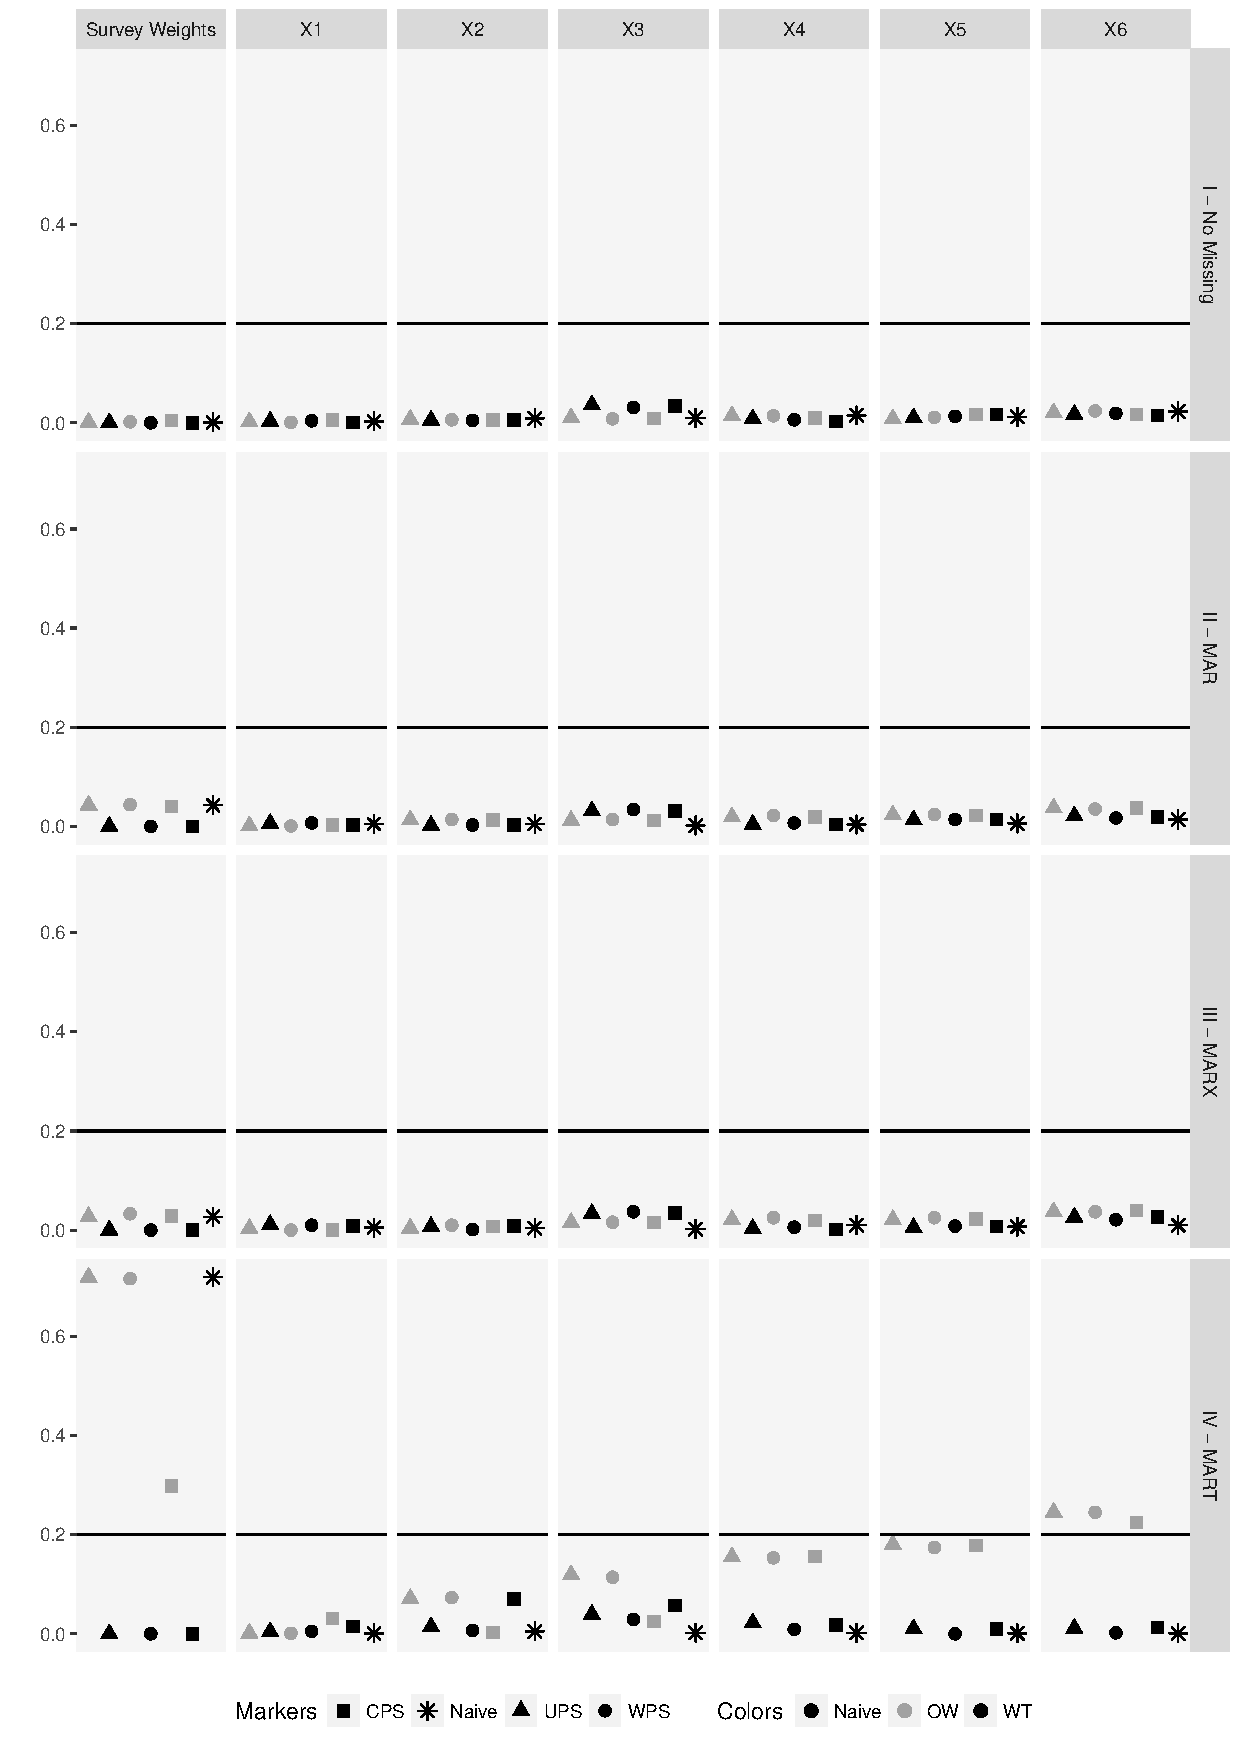
\includegraphics[scale=0.63]{SMD_SC1_v2.pdf}
\caption{{\small{}\textbf{Diagnostics: Scenario 1.} Average SMD computed in the matched samples in Scenario 1. Each marker represents how the survey weights were incorporated in estimation of the propensity score model: (\mytriangle{black}) survey weights were not used in the estimation of the propensity score model, but the sample weights are used in the computation of the SMD after matching, (\mycircle{black}) survey weights were incorporated in a weighted estimation of the propensity score model and (\mysquare{black})  survey weights were used as a covariate in the estimation of the propensity score model. Black markers are associated with the weight transfer described in Section \ref{S2.2}, gray markers show the balance achieved original survey weights are used. We also display the SMD achieved by the Naive estimator using a black asterisk.}}
\label{Diagnostics1} 
\end{figure}


\begin{figure}[t]
\centering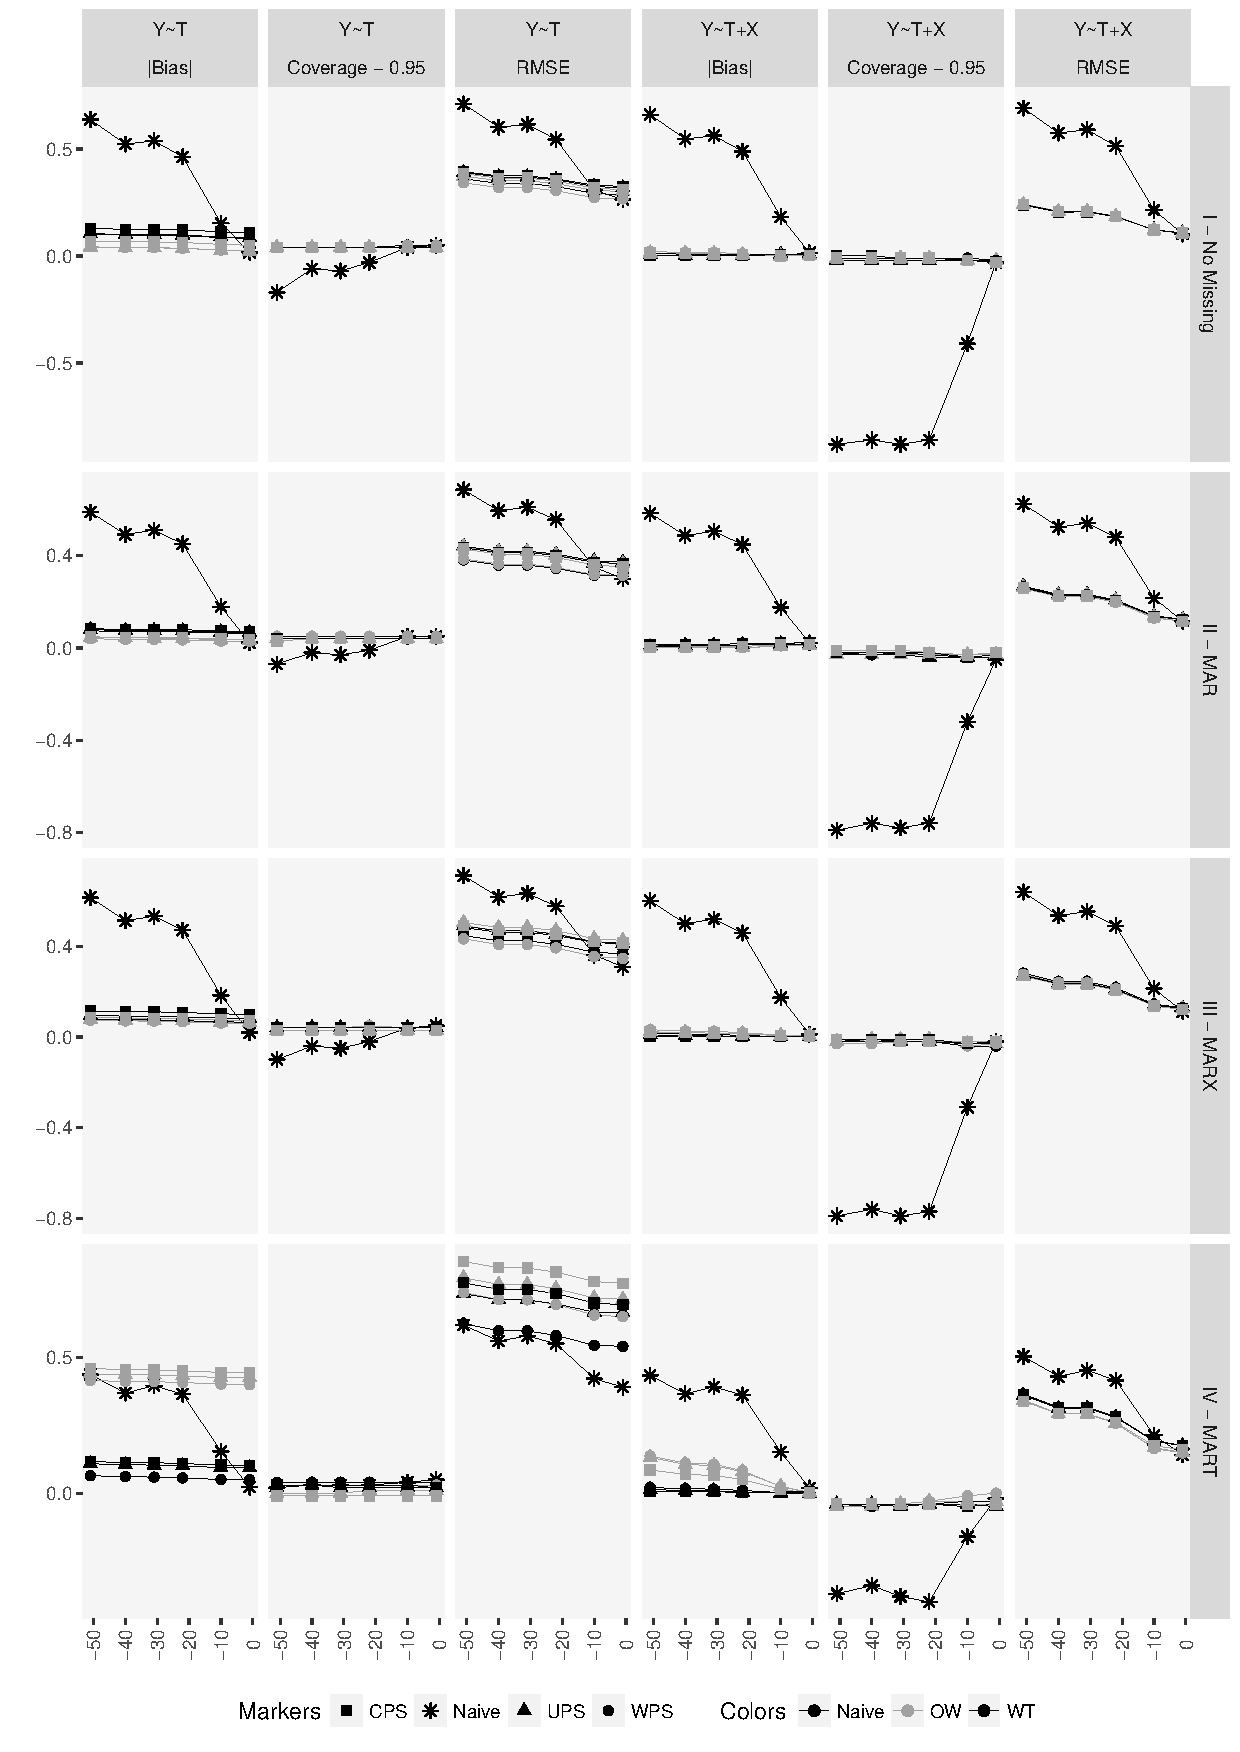
\includegraphics[scale=0.63]{Scenario1_v2.pdf}
\caption{{\small{}\textbf{Results: Scenario 1} Bias in absolute value, coverage and root mean squared error (RMSE) as functions
of the \% difference between the SATT and PATT (simulation study).Each marker represents how the survey weights were incorporated in estimation of the propensity score model: (\mytriangle{black}) survey weights were not used in the estimation of the propensity score model, but the sample weights are used in the computation of the SMD after matching, (\mycircle{black}) survey weights were incorporated in a weighted estimation of the propensity score model and (\mysquare{black})  survey weights were used as a covariate in the estimation of the propensity score model. Black lines  show the results when the wight transfer (see Section \ref{S2.2}) is implemented, gray lines show the results when the original survey weights are used. Results for the Naive estimator are displayed using a black asterisk.}}
\label{Scenario1} 
\end{figure}


\begin{table}[ht]
\centering
\caption{\textit{\small{}Standardized Mean Differences (Population level)} \label{Table 1}}
\begin{tabular}{rrrrrrr}
  \hline
Scenario & X1 & X2 & X3 & X4 & X5 & X6 \\ 
  \hline
1 & 0.11 & 0.28 & 0.43 & 0.49 & 0.69 & 0.81 \\ 
2 & 0.03 & 0.16 & 0.34 & 0.59 & 0.57 & 0.91 \\ 
3 & 0.09 & 0.22 & 0.33 & 0.48 & 0.60 & 0.81 \\ 
   \hline
\end{tabular}
\end{table}

\newpage
\begin{center}
\begin{longtable}{r|c|c|c|c|c|c|c}
\caption{SMD achieved by the different estimation procedures.} 
\label{Table 2} \\
\hline \multicolumn{1}{c|} {Variable} & 
	   \multicolumn{1}{c|} {Naive}    & 
       \multicolumn{1}{c|} {UPS$|$OW} & 
       \multicolumn{1}{c|} {UPS$|$WT} & 
       \multicolumn{1}{c|} {CPS$|$OW} & 
       \multicolumn{1}{c|} {CPS$|$WT} & 
       \multicolumn{1}{c|} {WPS$|$OW} & 
       \multicolumn{1}{c}  {WPS$|$WT} \\ \hline 
\endfirsthead

\multicolumn{8}{c}%
{{ \tablename\ \thetable{} -- continued from previous page}} \\
\hline \multicolumn{1}{c|} {Variable} & 
	   \multicolumn{1}{c|} {Naive}    & 
       \multicolumn{1}{c|} {UPS$|$OW} & 
       \multicolumn{1}{c|} {UPS$|$WT} & 
       \multicolumn{1}{c|} {CPS$|$OW} & 
       \multicolumn{1}{c|} {CPS$|$WT} & 
       \multicolumn{1}{c|} {WPS$|$OW} & 
       \multicolumn{1}{c}  {WPS$|$WT} \\ \hline 
\endhead

\hline \multicolumn{8}{r}{{Continued on next page}} \\ \hline
\endfoot

\hline \hline
\endlastfoot
  FEMALE & 0.08 & 0.08 & 0.06 & 0.08 & 0.06 & 0.03 & 0.01 \\ 
  WHITE & 0.05 & 0.05 & 0.05 & 0.05 & 0.05 & 0.10 & 0.14 \\ 
  WKSESL & 0.04 & 0.04 & 0.06 & 0.04 & 0.06 & 0.05 & 0.09 \\ 
  C1R4RSCL & 0.04 & 0.04 & 0.03 & 0.04 & 0.03 & 0.06 & 0.04 \\ 
  C1R4MSCL & 0.13 & 0.13 & \cellcolor[gray]{.9}0.24 & 0.13 & \cellcolor[gray]{.9}0.24 & 0.00 & 0.04 \\ 
  S2KPUPRI & \cellcolor[gray]{.9}0.25 & \cellcolor[gray]{.9}0.25 & 0.15 & \cellcolor[gray]{.9}0.25 & 0.15 & 0.01 & 0.02 \\ 
  P1ELHS & 0.02 & 0.02 & 0.04 & 0.02 & 0.04 & 0.02 & 0.10 \\ 
  P1EHS & 0.06 & 0.06 & 0.09 & 0.06 & 0.09 & 0.05 & 0.03 \\ 
  P1ESC & 0.10 & 0.10 & 0.08 & 0.10 & 0.08 & 0.02 & 0.00 \\ 
  P1EC & 0.15 & 0.15 & 0.09 & 0.15 & 0.09 & 0.13 & 0.04 \\ 
  P1EMS & 0.00 & 0.00 & 0.07 & 0.00 & 0.07 & 0.08 & 0.04 \\ 
  P1EPHD & 0.04 & 0.04 & 0.00 & 0.04 & 0.00 & 0.10 & 0.05 \\ 
  P1FIRKDG & 0.16 & 0.16 & 0.14 & 0.16 & 0.14 & \cellcolor[gray]{.9}0.20 & 0.17 \\ 
  P1AGEENT & 0.12 & 0.12 & 0.07 & 0.12 & 0.07 & 0.06 & 0.06 \\ 
  T1LEARN & 0.01 & 0.01 & 0.05 & 0.01 & 0.05 & 0.05 & 0.10 \\ 
  P1HSEVER & 0.03 & 0.03 & 0.03 & 0.03 & 0.03 & 0.03 & 0.16 \\ 
  FKCHGSCH & 0.00 & 0.00 & 0.09 & 0.00 & 0.09 & 0.05 & 0.12 \\ 
  S2KMINOR & 0.10 & 0.10 & 0.09 & 0.10 & 0.09 & \cellcolor[gray]{.9}0.21 & 0.12 \\ 
  P1FSTAMP & 0.02 & 0.02 & 0.13 & 0.02 & 0.13 & 0.05 & 0.14 \\ 
  SGLPAR & 0.05 & 0.05 & 0.07 & 0.05 & 0.07 & 0.04 & 0.17 \\ 
  TWOPAR & 0.05 & 0.05 & 0.07 & 0.05 & 0.07 & 0.04 & 0.17 \\ 
  P1NUMSIB & 0.06 & 0.06 & 0.01 & 0.06 & 0.01 & 0.07 & 0.12 \\ 
  P1HMAFB & 0.04 & 0.04 & 0.17 & 0.04 & 0.17 & 0.03 & 0.19 \\ 
  WKCAREPK & 0.03 & 0.03 & 0.14 & 0.03 & 0.14 & 0.06 & 0.06 \\ 
  P1EARLY & 0.07 & 0.07 & 0.09 & 0.07 & 0.09 & 0.05 & 0.09 \\ 
  P1WEIGHO & 0.06 & 0.06 & 0.11 & 0.06 & 0.11 & 0.05 & 0.09 \\ 
  C1FMOTOR & 0.14 & 0.14 & \cellcolor[gray]{.9}0.29 & 0.14 & \cellcolor[gray]{.9}0.29 & 0.13 & 0.11 \\ 
  C1GMOTOR & 0.15 & 0.15 & \cellcolor[gray]{.9}0.20 & 0.15 & \cellcolor[gray]{.9}0.20 & 0.06 & 0.07 \\ 
  P1HSCALE & 0.12 & 0.12 & 0.08 & 0.12 & 0.08 & 0.04 & 0.05 \\ 
  P1SADLON & 0.04 & 0.04 & \cellcolor[gray]{.9}0.22 & 0.04 & \cellcolor[gray]{.9}0.22 & 0.02 & 0.01 \\ 
  P1IMPULS & 0.09 & 0.09 & 0.17 & 0.09 & 0.17 & 0.02 & 0.06 \\ 
  P1ATTENI & 0.14 & 0.14 & \cellcolor[gray]{.9}0.23 & 0.14 & \cellcolor[gray]{.9}0.23 & 0.10 & 0.04 \\ 
  P1SOLVE & \cellcolor[gray]{.9}0.26 & \cellcolor[gray]{.9}0.26 & \cellcolor[gray]{.9}0.38 & \cellcolor[gray]{.9}0.26 & \cellcolor[gray]{.9}0.38 & \cellcolor[gray]{.9}0.20 & 0.14 \\ 
  P1PRONOU & 0.03 & 0.03 & 0.10 & 0.03 & 0.10 & \cellcolor[gray]{.9}0.28 & \cellcolor[gray]{.9}0.26 \\ 
  P1DISABL & 0.13 & 0.13 & 0.08 & 0.13 & 0.08 & 0.12 & 0.04 \\ 
  AVG4RSCL & 0.03 & 0.03 & 0.04 & 0.03 & 0.04 & 0.15 & 0.03 \\ 
  AVG4MSCL & 0.01 & 0.01 & 0.04 & 0.01 & 0.04 & 0.19 & 0.02 \\ 
  AVGWKSES & 0.03 & 0.03 & 0.06 & 0.03 & 0.06 & 0.14 & 0.03 \\ 
  C1\_6FC0 & 0.11 & 0.11 & 0.00 & 0.11 & 0.00 & 0.08 & 0.00 \\ 
\end{longtable}
\end{center}

\begin{table}[ht]
\centering %
\caption{PATT estimation. Unadjusted vs. Adjusted}{\textit{\small{}} \label{Table 3}}
\begin{tabular}{r |cc|cc}
\hline 
 & Unadjusted  & 95\% CI  & Adjusted  & 95\% CI \tabularnewline
\hline 
     Naive & -2.62 & (-4.44; -0.81) & -3.30 & (-5.98; -0.61) \\ 
  UPS$|$OW & -5.25 & (-8.55; -1.94) & -7.86 & (-13.42; -2.30) \\ 
  UPS$|$WT & -4.33 & (-7.24; -1.42) & -9.92 & (-14.98; -4.86) \\ 
  CPS$|$OW & -5.79 & (-8.98; -2.61) & -6.63 & (-12.18; -1.08) \\ 
  CPS$|$WT & -5.31 & (-8.39; -2.24) & -7.59 & (-12.89; -2.29) \\ 
  WPS$|$OW & -4.62 & (-8.05; -1.19) & -6.39 & (-11.90; -0.88) \\ 
  WPS$|$WT & -2.80 & (-6.13; 0.53)  & -5.97 & (-11.34; -0.61) \\
\hline 
\end{tabular}

\caption*{The first column displays the estimation result of implementing an unadjusted regression model and the second column shows the associated 95\% confidence interval. The third column, shows the results of estimating the PATT adjusting for the set of covariates considered in Table \ref{Table 2}, and the last column shows the associated 95\% confidence interval.}
\end{table}

\end{document}